\documentclass{article}
% set up the page formatting
\usepackage[a4paper, portrait, margin=2.5cm]{geometry}
\usepackage{multicol}
\usepackage{fancyhdr}
\usepackage{graphicx}
\usepackage{float}

% allow for table of contents to have clickable links
\usepackage{hyperref}

% editable bits
\title{\vspace{-1.5cm}CS261 Group 29 Final Report}
\author{Ani Bitri, Krister Hughes, Thomas Phuong, Eshan Sharif, Josh Turner, Antoni Zyla}
\date{January 2025 - March 2025}
\fancyfoot[L]{Final Report}
\fancyfoot[R]{\thepage}

\begin{document}
    \maketitle

    \tableofcontents

    \section{Preface}

    Dorset Software tasked our team with creating a traffic junction simulator.

    Dorset Software has tasked our team with the creation of a traffic junction simulator which will be used for the modelling of traffic junctions on various parameters. The system provides data on how these configurations
    affect the traffic flow and the overall efficiency of the junction in comparison to other configurations.

    This document explains the development process of the system and provide an explanation to the key changes and decisions made throughout the implementation of the prototype. Furthermore,
    it will give an insight into the algorithms and formulas used to calculate the traffic flow and efficiency of the junctions.


    \section{System Overview}

    \subsection{Purpose}

    Our system is a traffic junction simulator intended to be used by traffic engineers, urban planners and district governments to model and analyse the efficiency of different traffic junction configurations. The
    system includes a frontend interface for users to input their desired configurations, a simulation page to visualise the traffic flow and a results page to display the metrics of the simulation.

    \subsection{Developer Tools Used}

    The system was developed using Python and a few of its libraries. This allowed for easier transition between the frontend and backend of the system. The
    fronted was developed using PyQT5 for the GUI and MatPlotLib for aid in the Visualisation of the results.

    Our team also utilised GitHub for version control and better collaboration between team members.

    \subsection{User Interaction}

    The system is designed to be user-friendly and intuitive. When the application first opens, the user is greeted with the Home page where it displays the overview of the application and have the option to either exit to application or go to the "Input Parameters" page.
    page where they can input the desired parameters for the simulation.

    \subsection{System Architecture and Interaction}

    In the planning and design of the document it was decided that there would be a single point of contact between
    the frontend and backend portions, this has remained true. There is a single function which is called by the
    frontend to do all the computation. The frontend does use the data classes from the backend as a base for
    storing its data however they are not copied over but used as is so any modifications or refactoring would not
    require any major work.


    \section{Modifications}

    It turned out that the planning and design was not sufficiently detailed to properly create a fully functioning
    system just by itself, there were quite a few modifications required, some examples are listed below.

    \subsubsection{Backend}

    The backend had quite a few modifications, the planning and design document whilst a good start for the system was
    not fleshed out to the level required to implement a solution and make sure it was true to form. There are modifications
    in almost all data classes as well as the way they interact with each-other.

    For example we did not end up using a resultset class at all as it was necessary and just another layer between
    the data and it's usage. Passing it as raw data in a set of arrays was better for the frontend as they could
    directly iterate over it when drawing the graphs.

    More of these changes are listed later in the backend section of this file.

    \section{Frontend}

    \subsection{User Interface Design}
    The previous interface design combined the inputs, simulation, and results onto a single screen where you could tab between inputs and parameters. While this worked,
    a few issues arose when implementing it, such as, cluttered visuals, reduced usability, and a limited possibility of expansion. To address these newly found issues,
    instead of tabbing between the inputs and parameters pages, we made it so the inputs and parameters, the simulation, and results were given their own unique tab to
    function on. As a results of implementing the project this way, we found key advantages present in this layout compared to the previous one.

    \subsubsection{Improved Organisation}
    By separating the inputs, simulation, and results into distinct tabs, users can focus on one aspect of the interface at a time. This tabbed approach also enhances
    the workflow efficiency of the user and gives the user a natural progression to follow between data entry to simulation execution and results analysis.

    \subsubsection{Reduced Clutter}
    The previous design displayed all elements of our user interface on one screen, making it visually overwhelming and difficult to navigate. The new design split of
    the interface, allowing the user to interact with each section independently, reducing the visual overload and improving the overall ease of use.

    \subsubsection{Increased Space for Additional Features}
    The old layout restricted the ability of add new functionalities due to space constraints as all three segments were on one page. By utilising the tab-based system,
    we have created for room for additional features such as adding graphs to the results page.

    \subsection{Home Page}

    The user is first greeted with the home page where some general information about the system is displayed. The user can then click the "Go to Input Parameters" button to go to the Inputs Page
    or click the \("\)Exit\("\) button to exit the application.
    The image below shows the home page of the system:

    \begin{figure}[H]
        \centering
        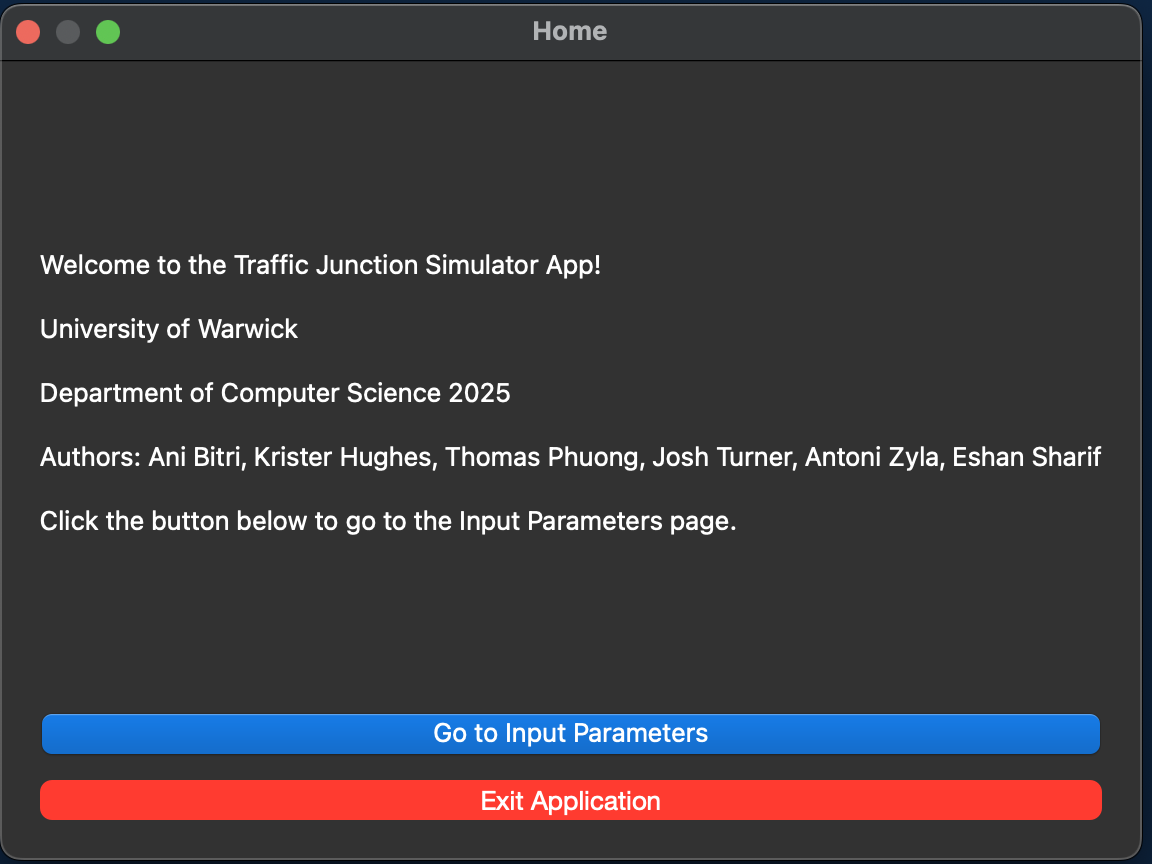
\includegraphics[width=11cm]{homepage}
        \caption{Home Page of the System}
        \label{fig:homepage}
    \end{figure}

    \subsection{Input and Validation Page}

    The Input Page provides a structured interface for configuring traffic flow conditions. The layout of the Input Parameters page made use of a grid and box layout to organise the input boxes for each junction. The widget uses PyQt's QScrollArea to allow the user to scroll through the multiple junction configurations, where each one of them
    is contained in a QGroupBox and stored as JunctionInputAndParameterWidget. Each JunctionInputAndParameterWidget contains 4 QGroupBoxes, one for each direction of traffic flow stored as RoadGroupWidget. Each RoadGroupWidget contains the input fields for the
    traffic flow, number of lanes, dedicated lanes, such as bus lanes and bus lane configuration, left turn lane and right turn lane; and also a priority input field. The image below shows the input page of the system:

    \begin{figure}[h!]
        \centering
        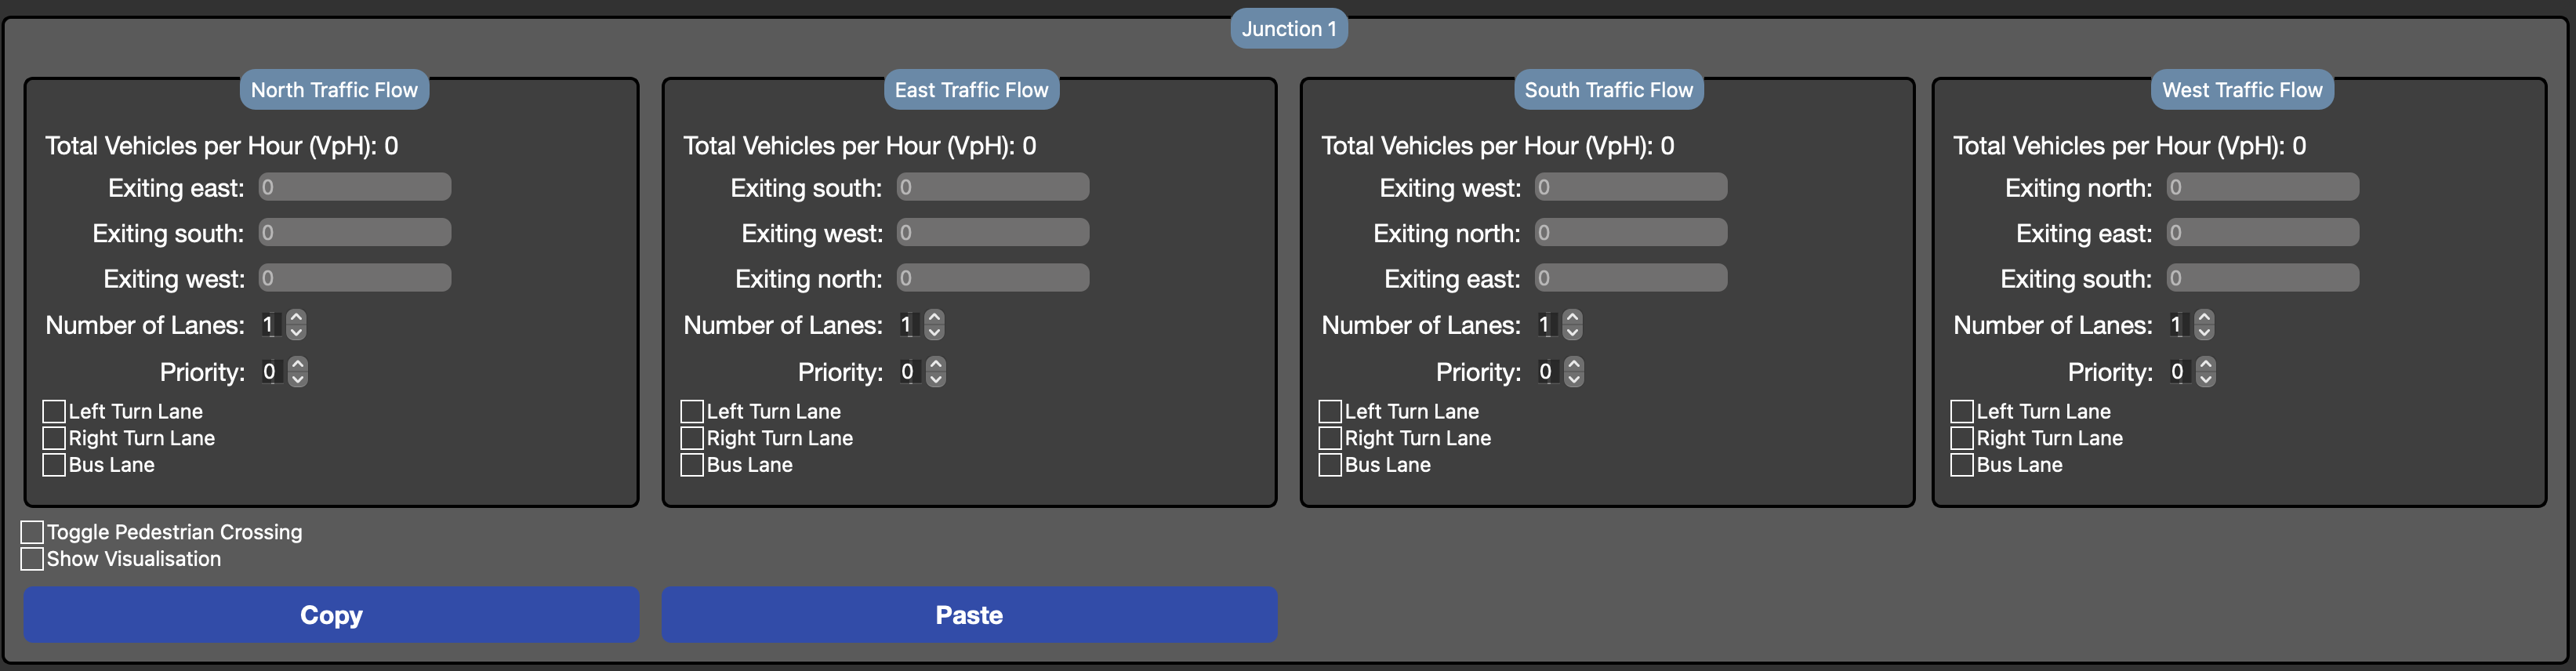
\includegraphics[width=\textwidth]{parameter}
        \caption{Illustration of the Input Box}
        \label{fig:parameter}
    \end{figure}

    The JunctionInputAndParameterWidget also contains two checkboxes for the user to select whether they want to add pedestrian crossing options and whether they want to see the updates on the junction on real time. A visual representation of the
    junction is displayed on the right side of the parent box, which updates in real time as the user inputs the parameters. Furthermore, the parent box contains copy and paste buttons, where the user can copy the data entered
    in the first junction configuration, and reuse it in the other configurations. The image below shows the visual representation:

    \begin{figure}[H]
        \centering
        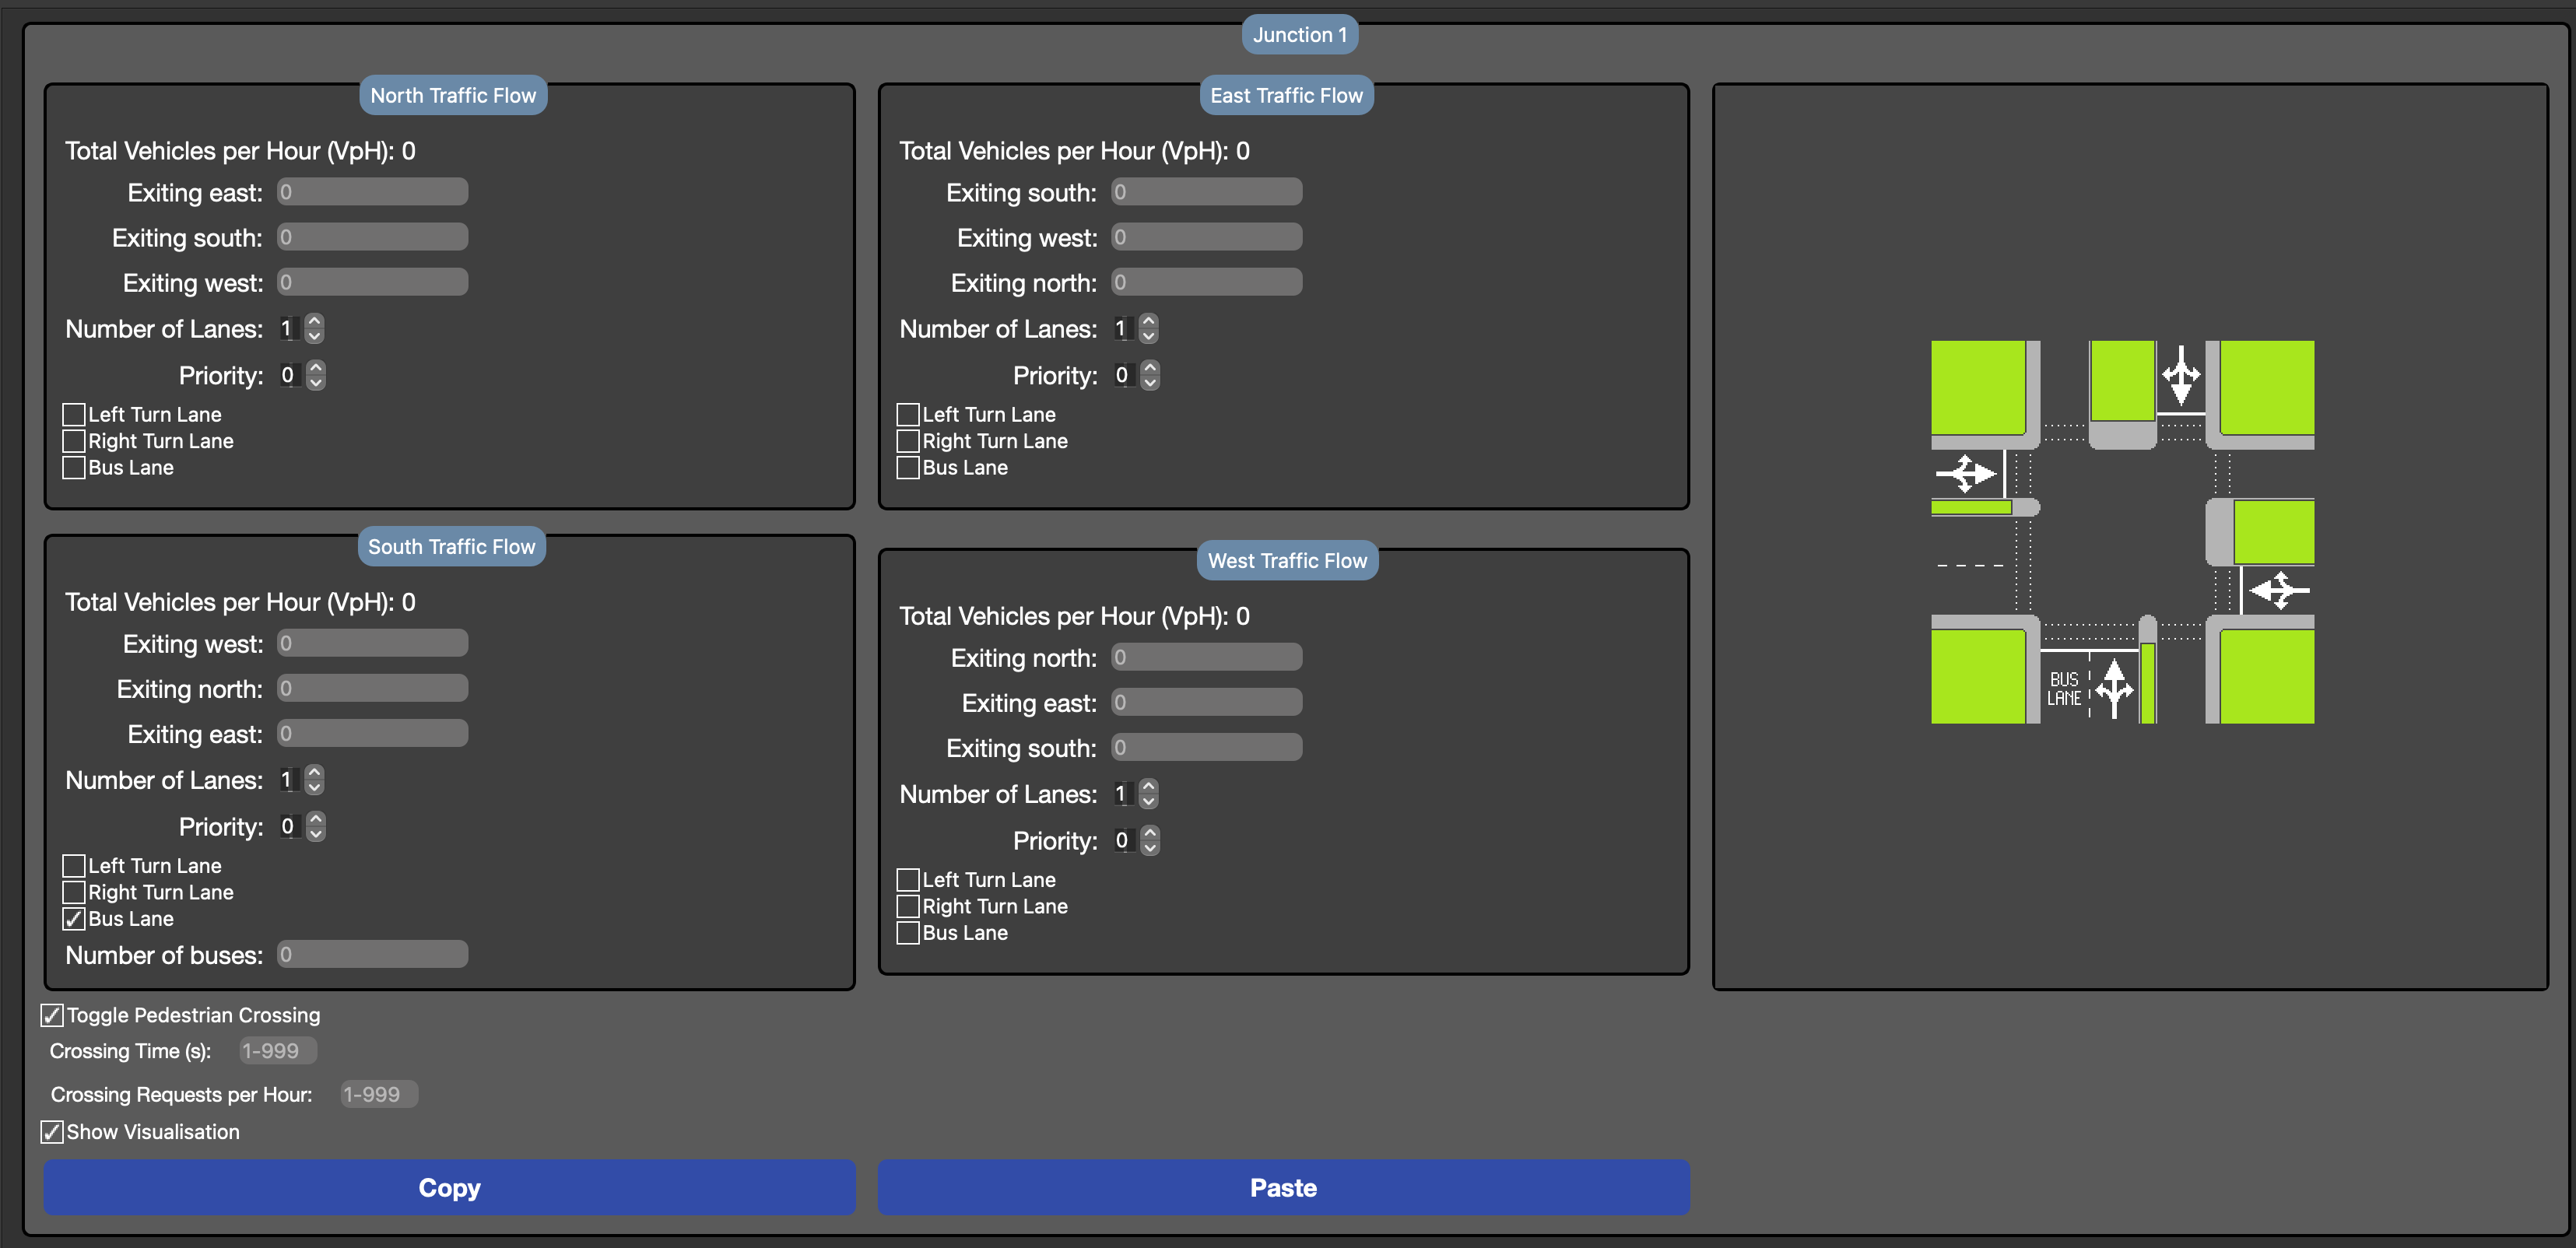
\includegraphics[width=\textwidth]{inputExtra}
        \caption{Illustration of the Input Box with additional options}
        \label{fig:inputExtra}
    \end{figure}

    Once the user has input the desired parameters, they can click the "Start Simulation" button at the bottom of the page to send the data to the backend and start the simulation. After the user has clicked the "Start Simulation" button, they
    will be taken to the Results Page where the results of the simulation will be displayed.

    \subsubsection{Visualisation}
    In the initial design document, the implementation of the junction visualisation was left fairly open to allow for future revisions, as permitted by the
    modified version of the Waterfall Methodology used by the group. Once a basic input window had been created, the constraints (Such as left lanes and bus
    lanes being mutually exclusive) on the junction became clearer; this then aided with the design of the classes involved:
    \begin{figure}[H]
        \centering
        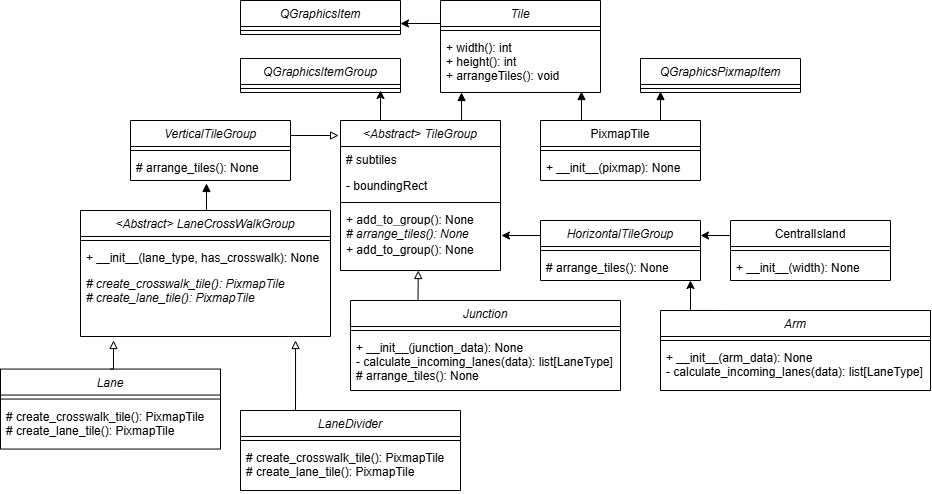
\includegraphics[width=\textwidth]{visualisation_class}
        \caption{Class diagram for the visualisation}
        \label{fig:visualisation_class}
    \end{figure}
    The overall structure was made to be hierarchical so that each layer could independently create and position the Tiles that they contained. Having both
    TileGroups and PixmapTiles inherit from Tile was intended to provide a layer of abstraction that would simplify the code.
    \begin{figure}[H]
        \centering
        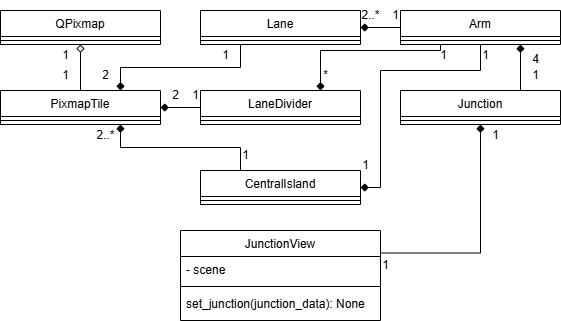
\includegraphics[width=0.6\textwidth]{visualisation_relationship}
        \caption{Relationships between classes in the visualisation}
        \label{fig:visualisation_relationship}
    \end{figure}
    When implementing this design for the visualisation, the team realised that it was inefficient to create a QPixmap for each tile in the image. This
    was because for some junction configurations there would be as many as one hundred and fifty QPixmaps created each time the junction was updated. To
    increase the efficiency, a class named Pixmap was created which held a single copy of each QPixmap. These QPixmaps are persistent between updates so
    only need to be created once when they are first used.\\

    The visualisation ended up meeting requirement 12 as it updates in real time as can be seen in the Dragon's Den video; however it was decided not to complete requirement 10 as this could have made the visualisation too cluttered, and could potentially be unintuitive to the user.

    \subsubsection{Copy and Paste}
    Although not in the origin design, the team decided to add copy and paste buttons as a quality of life improvement for the user.
    Before being implemented, comparing two junctions with the same flow rates required all twelve values to be copied manually from one junction to another; however, with the copy and paste button not only can these be copied with two clicks, but all other configurations for that junction are copied as well.
    This significantly improves the efficiency with which the user can compare two junctions with minor differences (Likely a common use case for this application).

    \subsection{Results Page}

    The Results Page initially displays a divided design using QGridLayout, a 2x2 grid where each cell is a QGroupBox planned to contain result information about the traffic flow for each direction, but initially,
    they display instructions on how the user can generate the results and how they will be displayed. The image below shows the initial state of a box in the results page:

    \begin{figure}[H]
        \centering
        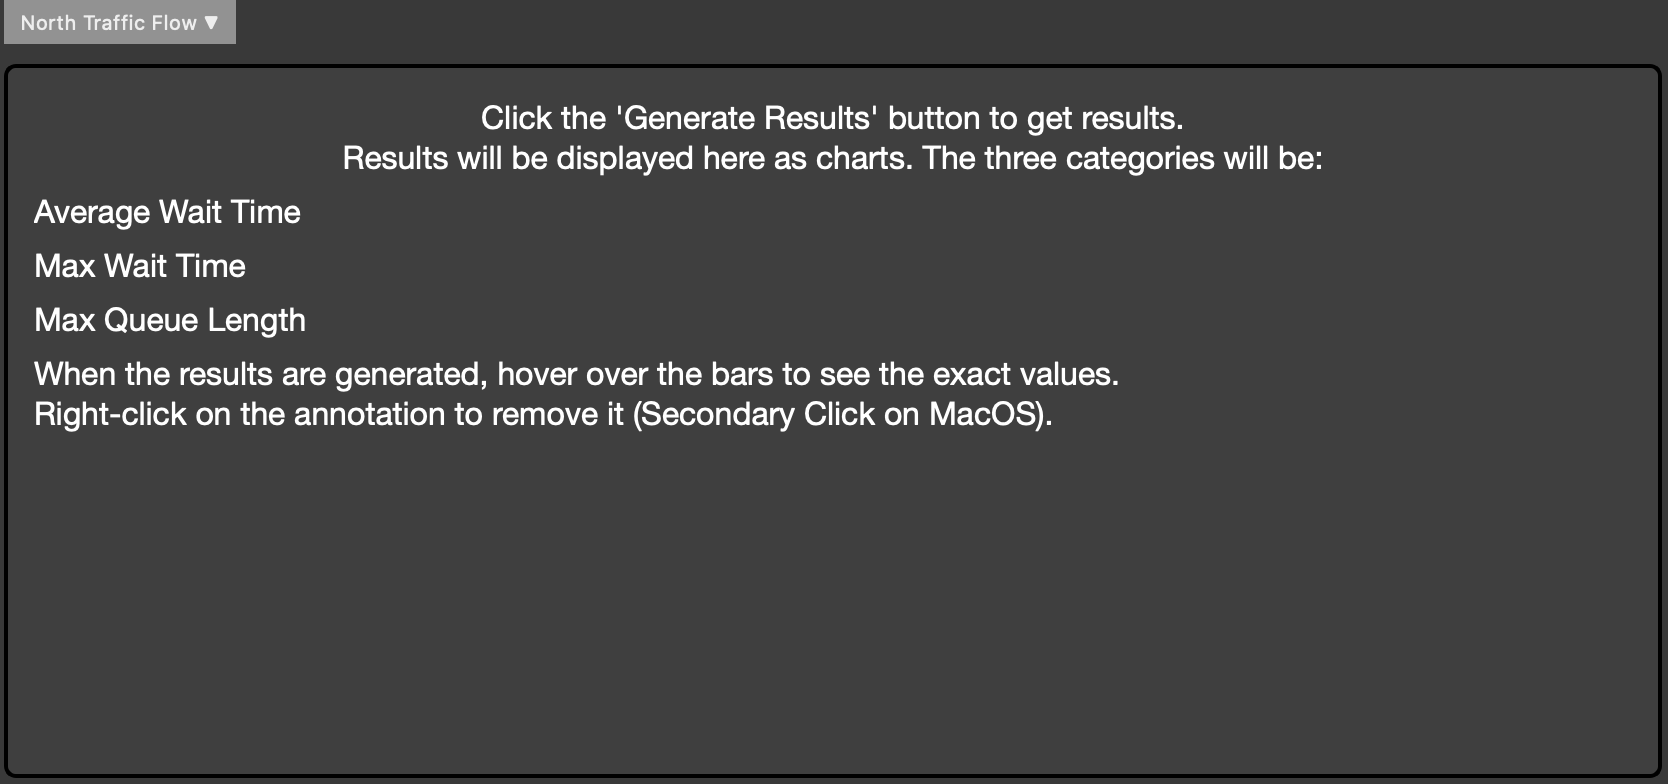
\includegraphics[width=\textwidth]{results1}
        \caption{Illustration of the initial state of a box in Results Page}
        \label{fig:results1}
    \end{figure}

    Once the user has generated the results, the boxes will display the metrics of the simulation on bar charts, where for the results categories (Max Queue Length, Average Wait, and Max Wait)
    each bar represents a different junction configuration. While the cursor is hovering over a bar, the user will be able to see the exact value of the metric. As instructed in the initial state
    of each direction box, the user can remove the annotation by right clicking over it (Secondary Click on MacOS). The image below shows the results page with the results of the simulation:

    \begin{figure}[H]
        \centering
        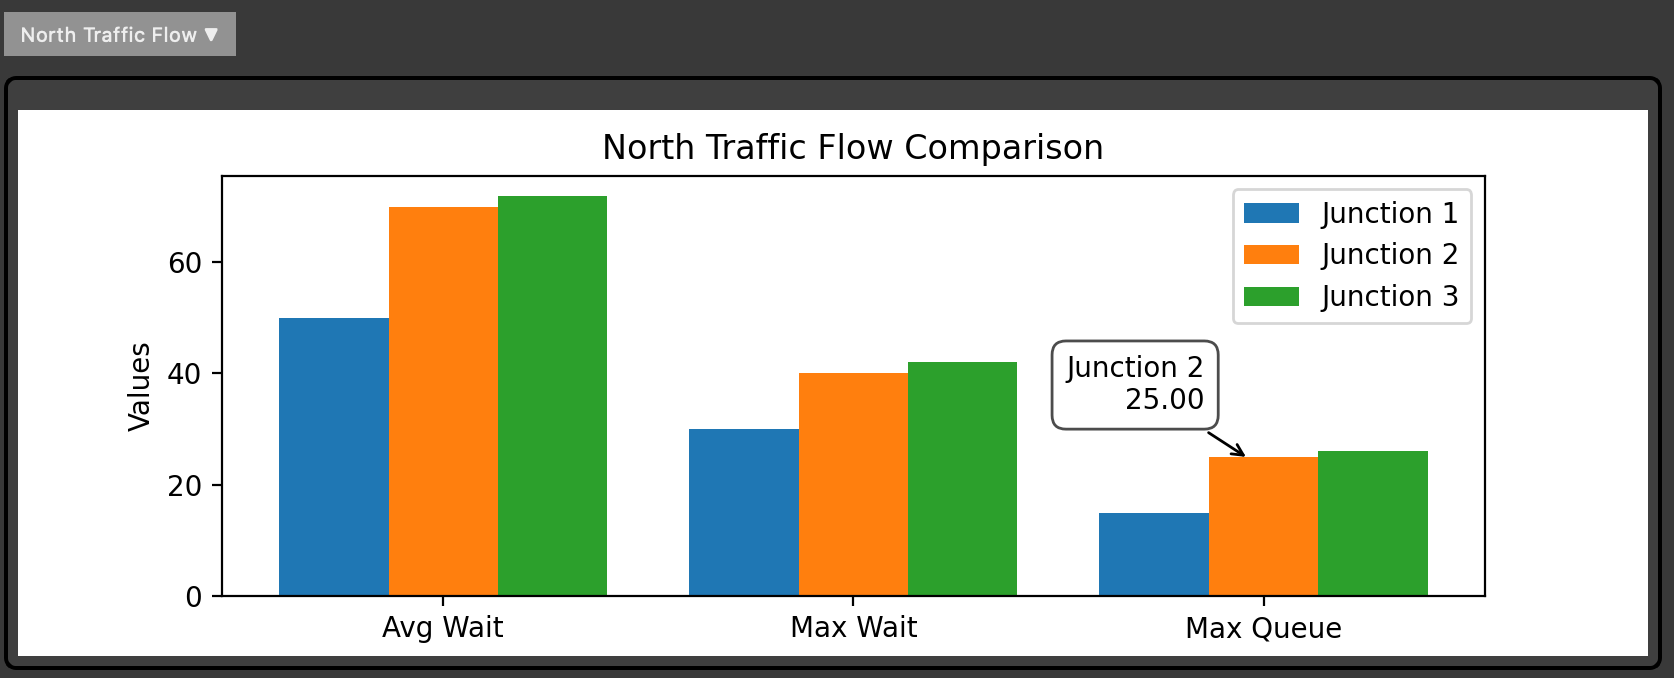
\includegraphics[width=\textwidth]{results2}
        \caption{Illustration of the chart with the results of the simulation for 3 different junction configurations}
        \label{fig:results2}
    \end{figure}

    The results set is retrieved as a 3D list from the backend, where the first dimension represents the junction configuration, the second dimension represents the direction of the traffic flow, and the third dimension represents the metrics. The overall scores
    for each junction are saved in the last index of the second dimension as a float.
    The image below represents the structure of the results set:

    \begin{figure}[H]
        \centering
        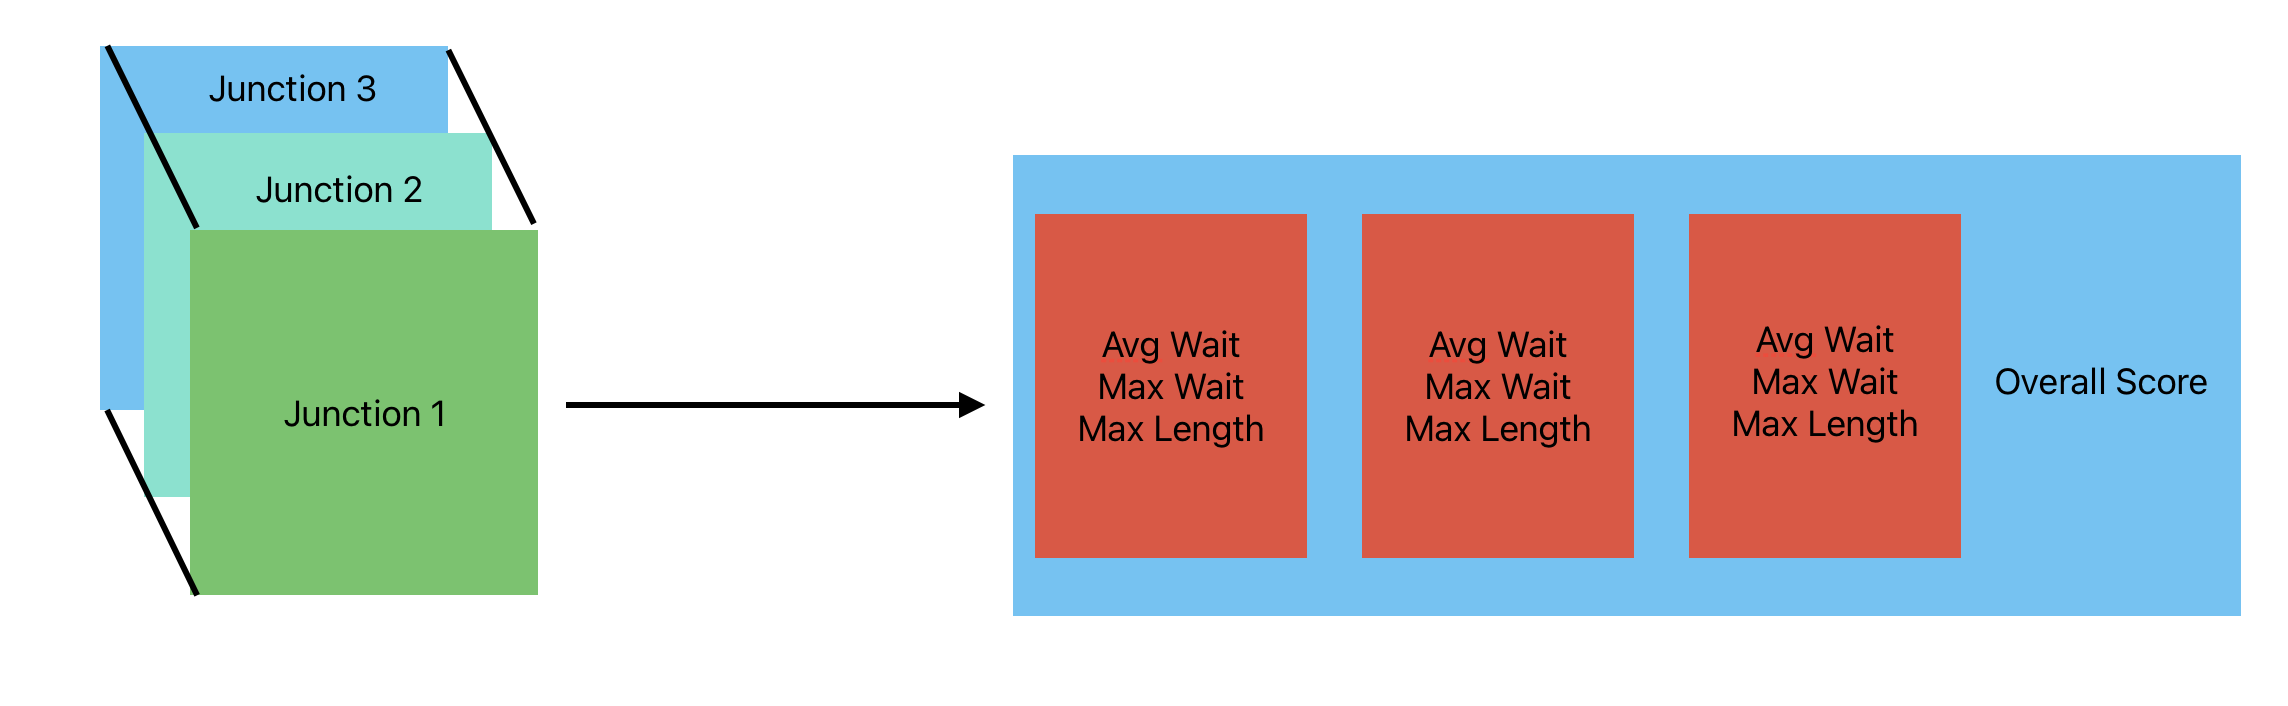
\includegraphics[width=\textwidth]{results3d}
        \caption{Illustration of result set structure}
        \label{fig:results3d}
    \end{figure}

    The overall scores for each junction configuration are also shown above the box layout of the directions. Depending on the number of junction configuration,
    the overall score labels will be adjusted accordingly to the layout of the page. The image below shows the results page with the overall scores displayed:

    \begin{figure}[H]
        \centering
        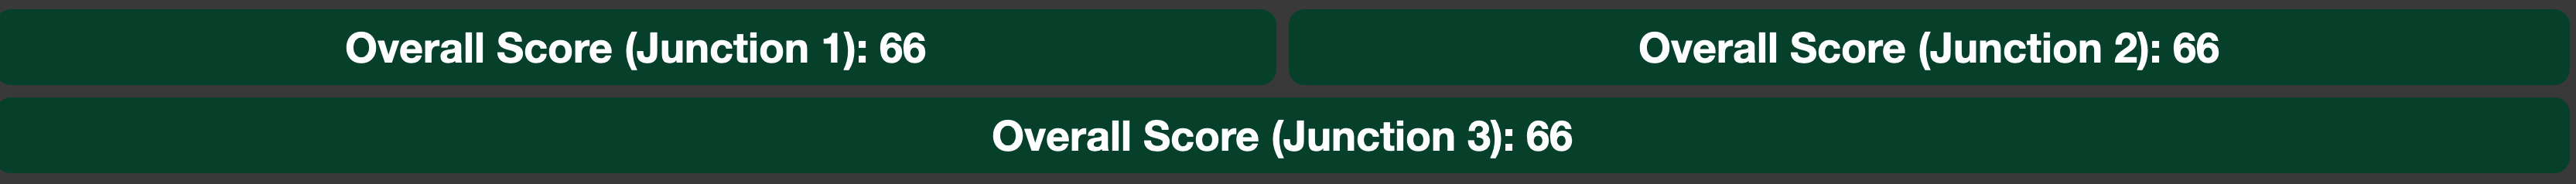
\includegraphics[width=\textwidth]{overallScores}
        \caption{Illustration of how the overall scores are displayed}
        \label{fig:overallScores}
    \end{figure}

    Furthermore, with the generation of the results, the user will also be able to generate a report PDF of the results. The user can do this by clicking the "Generate Report" button at the bottom of the page.
    The PDF report will contain the charts and the metrics for each direction in a text format. The next subsection will explain the PDF generation in more detail.

    \subsection{PDF generation}

    The PDF generation was implemented using the ReportLab library. It first checks whether the results have been generated (self.results\_generated). If the results exist, it prompts the user to choose a file
    location using a QFileDialog. If the user cancels the save operation, the function returns early. Otherwise, it ensures that the file has a .pdf extension before proceeding. The function then initializes a
    PDF canvas with an A4 page size and begins structuring the report by adding a title and introductory text. The function retrieves the results data from the get\_results() function and based on the number of junction
    configurations, it iterates over each direction to add a title and bar chart for each. The function then adds the overall scores and a final note before saving the PDF to the chosen file location.

    \begin{figure}[H]
        \centering
        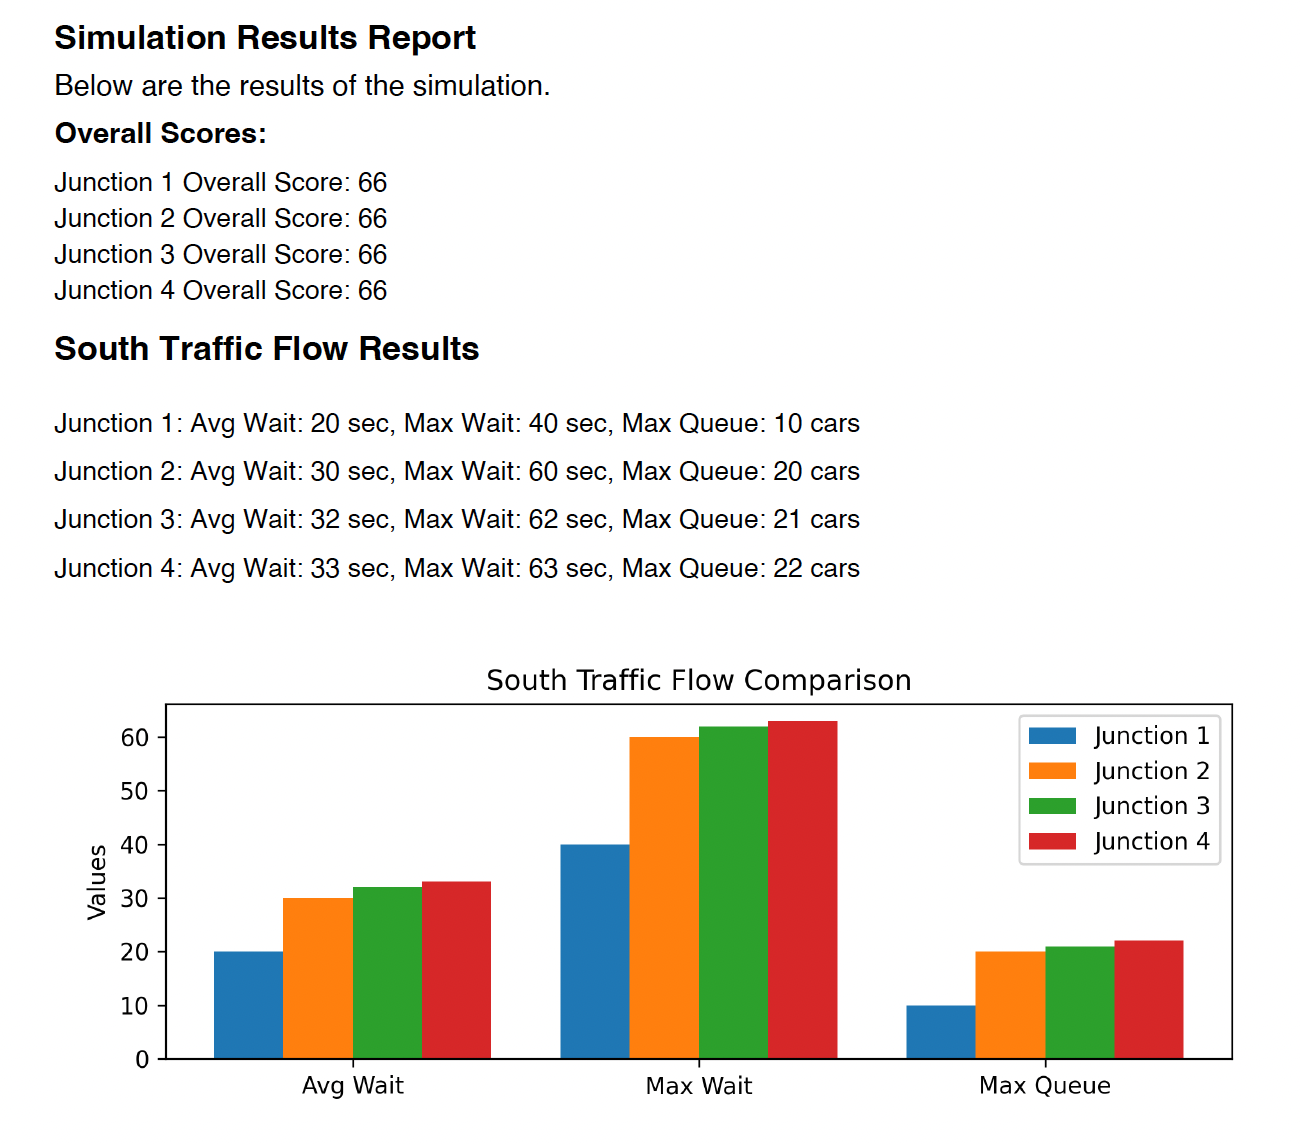
\includegraphics[width=\textwidth]{samplePDF}
        \caption{Sample of a PDF report generated by the system}
        \label{fig:samplePDF}
    \end{figure}

    \subsection{Error Handling}\label{subsec:error-handling}
    Within our application, there are many scenarios which require the user to input certain parameters or complete steps in a specific order. The way we handled these problems as a team were by checking and verifying the user's inputs by setting up certain constraints on the input boxes and by displaying error messages with the necessary steps to fix the issue on them.

    \subsubsection{Input Checking}
    On the Input and Parameter page we ensured that the user entered the correct inputs by having certain checks in place:
    \begin{itemize}
        \item When the user enters the VpH exiting each exit, we ensured that the input was an integer, greater or equal to 0, and had an upper bound of 999 VpH.
        \item When the user enters the number of lanes for each exit, the number had to be greater than 0, had an upper bound of 5, and was always an integer.
        \item For the Priority, we made sure that the user could only have a priority that was greater than or equal to 0, at most 4, and was an integer.
        \item If the user had chosen to add a pedestrian crossing, we made sure that the time it takes for people to cross and the number of crossing requests per hour were both greater than 0, less than 1000, and always an integer.
    \end{itemize}

    \subsubsection{Error Messages}
    There are features in our application that require the user to complete steps in a certain order.
    If the pre-requirement is not met for a certain feature, an error message will be displayed:

    \begin{figure}[H]
        \centering
        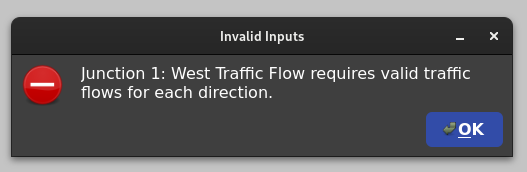
\includegraphics[width=0.7\textwidth]{example_error}
        \caption{Example of an error message displayed when an input is not entered}
        \label{fig:sampleError}
    \end{figure}

    \begin{itemize}
        \item If the user chooses to remove an alternate configuration without creating one in the first place, an error message will be displayed that will tell the user to add an alternate configuration before they are able to remove one.
        \item In the scenario that the user decides to generate a report PDF without generating any results, an error message would display: telling the user to press the generate results button in order to generate the results of their configuration before pressing the report button again.
        \item As the user is setting up their junction configuration, if the user does not set a suitable number of lanes, when starting the simulation an error message will display. The error message will prompt the user to change the number of lanes on the exit that has an inconsistent number of lanes and incoming traffic. The error message should tell the user which junction configuration is causing an issue and which direction of traffic flow needs to be changed.
    \end{itemize}


    \section{Backend}

    When implementing the backend we followed the class diagram and general structure as set out in the planning and
    design document, we encountered a few challenges once we got into the nitty-gritty implementation details, primarily
    regarding handling of the trafficlight timings for each lane and junction direction.

    \subsection{Data Classes}

    The system is split into the same classes as defined in the planning and design. However, during the development of the
    classes, we realised that the system hadn’t been considered thoroughly enough, so a lot of the methods and attributes
    inside the classes received changes.

    \subsubsection{Params and Flowrates}

    There was a slight modification of the final implementation of both of these classes compared to the initial class
    diagram, the flowrates object no longer contains a boolean variable for driving on either side of road as this was
    not able to be implemented in the timescale of the project. The planning design specifies the flowrates object to
    encapsulate the flow rates for all directions, we decided to use different flow rates object for each cardinal
    direction as this was simpler to program. The flow rates object also includes more data about dedicated left,
    dedicated right and dedicated bus lanes, with this comes a larger constructor as well as more getters for the
    flows derived from various combinations of the above. There is also a check function included in both classes to
    check that the data is of the correct format due to the lazy type system of python

    \subsubsection{Results Handling}

    In the planning and design it was intended to use an object \texttt{resultSet} to handle the passing of the result
    data from the backend to the frontend, this was deemed unnecessary, and instead we used raw data in a set of lists.
    This was easier not only for the backend to handle but also the frontend who could use the data directly when iterating
    over it whilst drawing the graphs in the frontend comparison function.

    \subsubsection{Junction, Vehicle, Direction, and Lane}
    For the Junction class, an accumulator attribute was introduced to implement pedestrian crossings: the accumulator would
    count the seconds since the previous pedestrian crossing started, pausing all directions traffic for the pedestrian crossing
    time when it became greater than the crossing rate per hour converted to seconds between crossings (3600 / crossing rate per hour)
    and then resetting to 0. The Vehicle class was updated with two extra attributes: time\_entered (discussed in the Results section) and
    type, used to indicate whether the vehicle is a car or a bus, used for implementing bus lanes.

    The implementation of run_simulation() in Junction - the main function in Junction - works as follows. The largest flow rate corresponding 
    to each traffic light setting (North-South Right, North-South Other, East-West Right, East-West Other) is calculated and then sorted from 
    largest to smallest. A for loop then runs for a set number of iterations, with the iterations cycling through the traffic light settings 
    in the sorted order previously determined. The number of simulation seconds a traffic light setting is on for is calculated by taking the 
    larger traffic light priority of the two directions indicated by the traffic light setting, adding 1 and then multiplying by 10. Then, the 
    Direction objects belonging to the Junction each have their simulateUpdate() method called, with the traffic light setting and simulation 
    seconds the setting is on for being passed in, after which add_to_pools() is called on all of the Direction objects to add the number of 
    vehicles that should have arrived during the time passed to the pools and/or lanes of the Direction. If the junction is configured to have 
    pedestrian crossings and a positive crossing rate per hour, then the accumulator’s value is considered at each iteration, skipping the calls 
    to Direction.simulateUpdate() when it reaches the threshold value mentioned earlier.

    Direction received major changes, having the pools changed from a list of counters to lists containing Vehicle objects (discussed further
    in the Results section), having the dedicatedLane and dedicatedLaneFlow attributes removed due to being handled by the FlowRates object.
    Direction also had a flows attribute added to store the flow rates corresponding to that road of the junction, as well as time\_elapsed,
    total\_cars\_exited, and cumulative\_time\_waited attributes, for the purposes of calculating the average wait. In terms of methods,
    simulateUpdate() was used for moving Vehicle objects out of Lanes, whilst a new method add\_to\_pools() was used for adding Vehicle objects
    to pools, where flow rates were divided by 3600 and multiplied by the number of simulation seconds to find out how many vehicles to add,
    with any fractional parts being stored in the residuals or bus\_residuals attributes (with vehicles being created the moment the cumulative sum
    of fractional parts exceed 1). Each of these also make a call to the method enqueue\_to\_lanes, which updates time\_elapsed as well as moving
    Vehicle objects from pools to lanes. Another method introduced was get\_total\_vehicles(), which returns how many vehicles are currently in
    that road of the junction (all vehicles in lanes + all vehicles in pools).

    Lane received the additional attributes is bus\_lane and maximum vehicle\_wait\_time, used for indicating whether the lane is a bus lane and
    keeping track of the maximum time a vehicle that exited that lane has had to wait for (used for calculating the maximum wait time in the 
    lane’s direction) respectively. The goes\_to() method returns whether one of the directions the lanes goes in is the direction passed in,
    while get\_queue\_limit() and get\_no\_available\_spaces() return the queue limit for the lane and how many more objects can be added to the
    lane with respect to the queue limit.

    The implementation of simulate\_update() in Lane - the main function in Lane - works as follows. The function is passed a list of directions,
    the time the traffic light setting is on for, and the current value of time\_elapsed from the Direction object it belongs to (see the Results
    section), and sets an internal variable called timer to the time the traffic light setting is on for. The function then repeatedly dequeues 
    Vehicle objects from the lane, decreasing the timer each time, until either the timer reaches 0, the lane is considered empty, or the next 
    vehicle to be dequeued is headed in a direction not in the passed list of directions. The first dequeued vehicle causes the timer to be decreased 
    by a decent amount, dependent on the direction the vehicle is headed, whereas all subsequent vehicles decrease the timer by 1, with the logic 
    being that these vehicles can be moving while the first vehicle is going through the junction, so don’t need to decrease the timer by the same 
    amount as the first vehicle. For each vehicle dequeued, the time that vehicle has waited for is added to a cumulative total for the purposes of 
    calculating the average wait time, and if the time waited by that vehicle is greater than the stored maximum time waited by a vehicle that was in 
    that lane, the maximum time is updated to the newly dequeued vehicle’s maximum wait time.


    \subsection{Simulation}

    For the simulation we utilised a top down nested structure. For example traffic light timing is generated in the
    junction class, passed down into the direction class and then from those individual lanes are set to be flowing
    or not based on where their vehicles are going and what their current traffic light is.

    This is all done synchronously and works based on working with non-intersecting paths, the left and ahead turns are
    all simulated for the same number of times in a given axis, then the right turn traffic. This allows us to not deal
    with the problem of cars in the junction at the same time or possible colliding paths.

    \subsection{Results}\label{subsec:results_backend}
    The results required to be displayed by the simulator per junction were the average wait time, maximum wait time and
    maximum queue length in each direction, along with an overall score for the junction. When implementing code to
    calculate the average wait time and maximum wait time for a direction, we realised that due to only representing a
    set number of vehicles in each lane as objects and the rest of the vehicles via counters in a list called pools
    (each counter corresponding to a direction a vehicle may exit), calculating the average wait and maximum wait would
    be difficult and we could only get an approximation - vehicles couldn’t store how long they had actually been waiting,
    since they were initially represented as part of a counter. This led us to the decision to rewrite the pools from being
    a list of counters for the number of vehicles outside the Lane objects heading in each direction, to each pool being
    a list containing Vehicle objects, all headed in the direction the pool was designated to. Along with this, the Vehicle
    class was updated to contain a time\_entered attribute, a timestamp indicating what time it arrived to the junction,
    and each Direction object had a time\_elapsed attribute (indicating the time in simulated seconds since the start of
    the simulation) to compare time\_entered to in order to work out how long a vehicle had been waiting. This was chosen
    over each vehicle having a timer keeping track of how long it had been at the junction for, since this would have
    required updating every Vehicle object every time Direction.simulateUpdate() was called, which for large flow rates
    would lead to a large amount of computation for each call, slowing the simulator down significantly.

    For the overall score, after working on it as a group, we came up with the following equation:
    $$score(J) = \sum_{d \in Dirs}\frac{flow(d) + k_P\times crossTime(d) \times crossRate(d)}{k_W (meanWait(d)+\frac{(maxWait(d))^2}{meanWait(d)}) + k_L\times maxLength(d)}$$
    The reasoning for making it dependent on the flow rate of each direction was because if a junction achieves a specific set of metrics (excluding overall score) for each direction with a certain set of flow rates, but another junction achieves that same set of metrics with a set of higher flow rates, then that second junction must be better and therefore receive a higher score. We decided to include crossing time and crossing rate in the equation since otherwise including pedestrian crossings would always lower the overall score due to preventing any traffic from flowing at given points, and in real life, pedestrian crossings do have value despite reducing how often traffic can flow. Since the score should reduce as average wait, max wait and max length increase, we decided to divide the flow rate and pedestrian crossing adjustment by average wait and max length, as well by max wait multiplied by max wait over average wait. Max wait was multiplied by this since we thought max wait should have more significance the further the value gets from average wait - for example, a junction with an average wait of 1 minute but maximum wait of an hour isn’t a very good junction. The equation also includes constants to allow for fine-tuning to prefer certain junction configurations over others.


    \section{Testing}

    \subsection{Unit Testing}
    Unit testing was a crucial step in ensuring the accuracy and reliability of the traffic simulation system. By testing components in isolation before integrating them, we identified and resolved potential issues early. This approach validated the system’s functionality under various traffic conditions, ensured stable performance when handling large datasets, and prevented erroneous behaviours caused by unexpected inputs.

    \subsection*{Junction Class}
    The \texttt{Junction} class simulates traffic flow at intersections, managing vehicle movement and traffic light sequencing.
    \begin{itemize}
        \item The system dynamically adjusted traffic light sequencing based on real-time traffic demand. Testing confirmed that high-traffic lanes received extended green-light durations, while conflicting signals were never activated simultaneously. The logic correctly prioritised heavy-flow directions while preventing unnecessary delays for lighter-traffic lanes.
        \item Vehicle movement was simulated to verify congestion patterns, ensuring that throughput calculations reflected realistic travel times. Tests confirmed that vehicle counts decreased appropriately as cars exited the junction and that waiting times increased proportionally with higher traffic density. Data logging ensured accurate tracking of each vehicle’s journey from arrival to departure.
    \end{itemize}

    \subsection*{Lane Class}
    The \texttt{Lane} class handles vehicle queues and determines progression based on traffic signals.
    \begin{itemize}
        \item Lane capacity constraints were rigorously tested to confirm that vehicles queued in a structured manner, preventing unintended bypasses or unrealistic pile-ups. Simulations verified that vehicles moved forward only when the traffic signal allowed, with proper prioritisation for left, right, and straight movements based on sequencing rules.
        \item Empty lane optimisation was validated to ensure that the system did not perform unnecessary calculations for lanes with no vehicles. Conversely, in full-capacity scenarios, vehicles were correctly held in place until space became available, preventing system crashes or skipped queue positions.
    \end{itemize}

    \subsection*{Parameters Class}
    The \texttt{Parameters} class manages key simulation settings, including lane numbers, pedestrian crossings, and sequencing priorities.
    \begin{itemize}
        \item Input validation was tested extensively, rejecting negative lane counts, sequencing priorities outside the expected range (0-4), and unrealistic pedestrian crossing times exceeding safe thresholds. The system consistently returned appropriate error messages for incorrect inputs, ensuring that invalid configurations did not proceed to simulation.
        \item Dynamic updates to parameters were tested by modifying settings mid-simulation. The system correctly adjusted sequencing priorities, lane capacities, and pedestrian timings in real time without disrupting existing traffic states. This confirmed that parameter modifications seamlessly influenced traffic flow without requiring a system restart.
    \end{itemize}

    \subsection*{FlowRates Class}
    The \texttt{FlowRates} class defines vehicle arrival rates and enforces lane-specific traffic rules.
    \begin{itemize}
        \item The system correctly rejected negative vehicle flow rates and prevented excessively high values from distorting congestion levels. Tests confirmed that each lane’s turn restrictions were respected, ensuring that right-turn-only lanes did not process straight-traveling vehicles and vice versa.
        \item Stress testing simulated extreme cases, including intersections with zero traffic and junctions with over 1000 vehicles per hour in a single direction. The system maintained stable performance, ensuring that congestion did not overflow into unrealistic queue lengths and that vehicle processing remained within expected real-world limits.
    \end{itemize}

    \subsection*{ResultSet Class}
    The \texttt{ResultSet} class stores final simulation outputs, including traffic efficiency metrics and vehicle throughput.
    \begin{itemize}
        \item Tests verified that simulation results, such as total vehicles processed, congestion levels, and average wait times, were logged correctly for each road direction. The system consistently produced structured reports with clear, interpretable metrics, allowing for accurate comparison of different traffic configurations.
        \item Edge cases such as complete traffic stagnation were tested to confirm that efficiency scores accurately reflected congestion severity. Additionally, extremely high efficiency values were examined to ensure proper formatting and that numerical overflows did not cause incorrect or misleading results.
    \end{itemize}

    \subsection*{Conclusion}
    Thorough unit testing ensured that all core components functioned correctly before full integration. By systematically validating sequencing logic, queue management, flow rate handling, and simulation outputs, we eliminated potential inconsistencies and performance issues. Identifying and resolving errors early improved system reliability, minimised unexpected failures, and ensured that edge cases—such as gridlocked intersections, empty roads, and misconfigured parameters—were handled correctly. The results confirmed that the system can adapt to real-world traffic conditions while maintaining stability, accuracy, and efficiency.

    \subsection{User Testing}

    The majority of the testing for the frontend was via the use of user testing, any changes made in the code were immediately
    reflected in the frontend visually

    \subsection{Error Handling Testing}
    \begin{itemize}
        \item Precondition Testing
        \begin{itemize}
            \item Ensured that error messages were displayed when prerequisites for actions were not met:
            \begin{itemize}
                \item When attempting to remove an alternate configuration without having created one, an error message is displayed prompting the user to add one first.
                \item When attempting to generate a report PDF without first generating results, an error message is displayed informing the user to generate results before generating a report.
                \item when Attempting to start the simulation when the lanes aren't balanced with the traffic, the error message should always be raised.
            \end{itemize}
        \end{itemize}
        \item Sequence Testing
        \begin{itemize}
            \item Validated that the correct error messages were triggered when users followed incorrect sequences of actions:
            \begin{itemize}
                \item Attempting to start the simulation without setting a suitable number of lanes triggers an error message specifying the exit lane inconsistency.
                \item Attempting to generate a report without generating results triggers an error message instructing the user to press the generate results button first.
                \item Attempting to remove an alternate configuration before generating an alternate configuration should raise the error.
            \end{itemize}
        \end{itemize}
        \item Consistent Testing
        \begin{itemize}
            \item Checked that error messages were consistently displayed for the same type of error across different scenarios:
            \begin{itemize}
                \item If an exit lane configuration is inconsistent with incoming traffic, the error message always specifies which direction of traffic and which exit are causing the issue.
                \item Made sure the error message when removing an alternate configuration only happened when there were 0 alternate configurations generated.
                \item Made sure that the error message was always displayed if the user tried to generate a report before trying to generate any results
            \end{itemize}
        \end{itemize}
    \end{itemize}

    \subsection{Input Checking}

    \begin{itemize}
        \item Boundary Testing
        \begin{itemize}
            \item Tested inputs on both the lower and upper bounds for the valid ranges:
            \begin{itemize}
                \item For VpH, tested the range 0-999 to ensure values within this range are accepted.
                \item For the number of lanes, tested the range 1-5 to ensure values within this range are accepted.
                \item For priority levels, tested the range 0-4 to ensure values within this range are accepted.
                \item For pedestrian crossing time and number of requests per hour, tested the range 1-999 to ensure values within this range are accepted.
            \end{itemize}
        \end{itemize}
        \item Erroneous Testing
        \begin{itemize}
            \item Tested with non-integer inputs (e.g., strings like "abc" or decimals like 2.5) to ensure only integers are accepted.
            \item Tested with invalid characters (e.g., special characters like "@\#\$") and blank spaces to ensure they are rejected.
            \item Tested values just outside the allowed range (e.g., -1 for VpH, 0 for number of lanes, and 6 for priority) to ensure they are not accepted.
        \end{itemize}
    \end{itemize}


    \section{Product Evaluation}

    The system meets the majority of the requirements we outlined previously, it meets all the must requirements and
    most of the should requirements.

    \begin{figure}[H]
        \begin{center}
            \begin{tabular}{ |c|p{9cm}|c| }
                \hline
                Requirement & Tests                                                                                               & Result \& Justification        \\
                \hline
                1C          & Flow rates added using the UI                                                                       & Passed - User Test             \\
                \hline
                2C          & Toggle Lane Numbers, Left Lane, Right Lane, Bus Lane and Pedestrian Crossings assigned using the UI & Passed - User Test \\
                \hline
                3C          & Priority Values for lanes can be assigned using the UI                                              & Passed - User Test             \\
                \hline
                4C          & User Will have a graphical representation of the junction                                           & Passed - User Test             \\
                \hline
                5C          & User Will be able to create multiple Junction Configurations and simulate simultaneously & Passed - User Test \\
                \hline
                6C          & User Will be presented with statistics about the Junction's performance                             & Passed - User Tested           \\
                \hline
                7C          & The User will be given the Overall Score + 6C Results in a tabular format                           & Passed - User Tested           \\
                \hline
                8C          & The User should be able to select the side of road that cars drive on                               & Failed - Not implemented       \\
                \hline
                9C          & The system should take into account the distance a car needs to travel in the junction & Failed - Not Implemented Fully \\
                \hline
                10C         & The user should be able to view the flow from any arm of the junction in a Sankey Diagram & Failed - Not Implemented \\
                \hline
                11C         & The User Must be provided with user friendly messages on system failure or error & Passed - User Test \\
                \hline
            \end{tabular}
            \caption{Customer Facing Requirements Tested}
        \end{center}\label{fig:figure}
    \end{figure}

    \begin{figure}[H]
        \begin{center}
            \begin{tabular}{ |c|p{9cm}|p{5cm}| }
                \hline
                Requirement & Description & Tested \\
                \hline
                12 & Graphical Representation should respond to input changes in under 0.5 seconds & Passed - Instantaneous updates \\
                \hline
                13 & Run on Linux, Mac and Windows & Passed - Developed and ran on all 3 \\
                \hline
                14 & Modular and Well documented & Borderline - Modular but not fully documented \\
                \hline
            \end{tabular}
            \caption{Non Functional Requirements Evaluated}
        \end{center}\label{fig:figure2k}
    \end{figure}

    \subsection{Deployment}

    The project is provided with an instructions file \texttt{command.txt} which has instructions for running the
    project, installing any necessary libraries.
    There are also compiled executables for Linux and Windows provided in the git repo.

    We did want to use docker to have a consistent build environment however this proved challenging as only one person
    on the team actually used a linux computer every day and would have required everyone else to use virtualised solution.
    We also felt that it was out of the scope of a basic project to include docker when the requirements for packaging were
    still unknown.

    \subsection{User Feedback}

    We managed to get feedback from a few users who tested a prototype of the system. The feedback was generally positive with users finding the system easy to use and understand. However, there were a few suggestions for improvements:

    \begin{itemize}
        \item One user suggested that the system should have a feature to save the results of the simulation in a database so that they can be accessed at a later time.
        \item Another user suggested that the system should have a feature to save the junction configurations so that they can be loaded at a later time.
        \item It was also suggested that the system be should have a feature to alternate between different types of junctions.
    \end{itemize}

    \subsection{Future Improvements}

    Implementing a database or a way to save configurations and their results to a file would be a good way of improving
    the system. Users would be able to save their work and come back to it if they could not complete it in a single
    session and would prevent them having to write results down and come back to them. It would also allow for easier
    testing of the consistency of the system over a larger period time and number of updates.

    Implementation of different junction types such as roundabouts or more complex 3 or 5 way junctions would be something
    that would be very useful to implement in the future. This would expand the size of the market that would make use
    of the software.

    Not mentioned by user testing, but we could implement the ability to find an optimal junction layout for a set of
    flow rates and certain restrictions, e.g. 150 vehicles per hour in all directions but can only have 3 lanes North and
    2 in the other directions, the system would then find the optimal layout and suggest to the planner.

    \section{Process Evaluation}

    \subsection{Time Management}

    Due to unforeseen circumstances, one of our group members could not contribute to the project as much as they would have liked to. This meant that the rest of the group had to distribute 
    the work between the remaining members. Since the work was being distributed, we had to reevaluate our time management strategy to make sure that the work was being done.
    We increased the number of meetings we had per week to make sure that the work was being done and that everyone was on the same page.  Additionally, we prioritised task delegation based on each member’s strengths
    and availability to ensure an efficient workflow. This approach allowed us to distribute the workload fairly while maintaining productivity. To track our progress, we utilised project management tools to document
    completed tasks, pending work, and any challenges faced. By increasing communication and adapting our strategy, we were able to mitigate the impact of the unforeseen circumstances. Regular check-ins helped us identify potential 
    bottlenecks early, allowing for quick resolution. Despite the unexpected challenge, our ability to collaborate effectively and adjust our approach ensured that we remained on track to complete the project successfully. The image 
    below shows a Gantt chart of the project timeline:

    \begin{figure}[H]
        \centering
        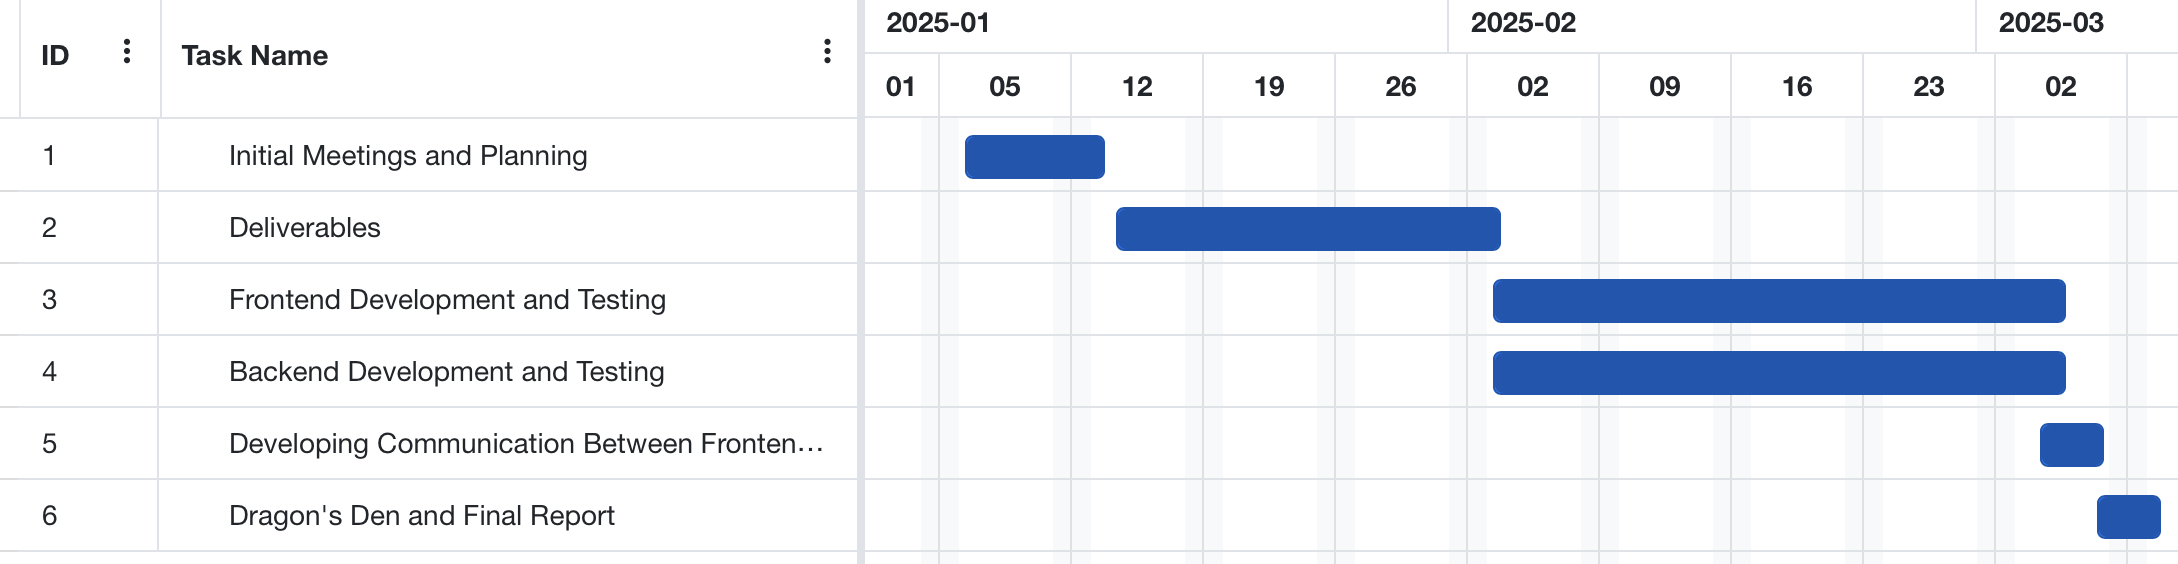
\includegraphics[width=\textwidth]{ganttChart}
        \caption{The Gantt Chart of the project timeline after the reevaluation of the time management strategy}
        \label{fig:ganttChart}
    \end{figure}

    \subsection{Methodology Feasibility and Evaluation}

    As outlined in our Planning and Design document, we opted for a slight variation of the Waterfall methodology, incorporating incremental development and reuse methodologies. This approach allowed us to maintain a structured 
    development process while retaining some adaptability to reevaluate requirements and design midway through the project if new needs arose. We chose this methodology due to its clear phase-based structure, which provided 
    organisation and direction, while the incremental aspect ensured that we could validate progress at multiple stages. Given our limited development timeframe, this hybrid approach balanced the predictability of Waterfall
    with the flexibility needed to handle any unforeseen changes efficiently.

    Having completed the development phase, we believe that our methodology choice was well-suited to our project. The structured nature of Waterfall helped us establish clear milestones and manage our resources effectively, 
    ensuring that each phase was well-defined and completed before moving forward. However, the ability to reassess requirements mid-development proved crucial, as it allowed us to accommodate necessary refinements without major 
    disruptions. Additionally, the reuse methodologies we incorporated helped streamline development, reducing redundant work and allowing us to focus more on system functionality. This approach was particularly beneficial given 
    our team’s initial unfamiliarity with large-scale software development, as it ensured a clear framework while still allowing for course corrections.

    That said, we did encounter some limitations with our methodology. The sequential nature of Waterfall made it challenging to accommodate last-minute changes efficiently, and while our incremental approach mitigated some of these 
    issues, we occasionally found ourselves constrained by the rigidity of predefined phases. Furthermore, although reuse methodologies helped speed up development, they also required careful integration and testing to ensure consistency 
    across components. In hindsight, a more iterative agile approach might have provided greater flexibility in addressing evolving requirements, though it would have required a higher level of adaptability from the team.

    Overall, we believe that our chosen methodology was a feasible and effective choice given the nature of our project. It provided structure and clarity while allowing for necessary adjustments, ultimately ensuring the timely 
    delivery of a functional product. However, future projects with similarly tight timelines and evolving requirements might benefit from an approach that incorporates even more iterative elements, such as a hybrid Agile-Waterfall 
    methodology, to maximize both adaptability and efficiency.

    \subsection{Key Strengths and Limitations}

    Overall, our team is of the opinion that our project was mostly successful. The aspect of communication and team coordination was a crucial part of the project, and we believe that we did well in that aspect. The team was able to overcome the
    challenges that arose during the project and through re-distribution of the workload and good communication, we were able to complete the project on time. Another key aspect that aided the development of the project was the division of the group 
    into roles. This allowed for a more efficient workflow as each person had a specific role to do and could focus on that. Our strong initial meeting and planning phase also helped us to stay on track and complete the project on time. We were able to
    identify potential issues early on and address them before they became a problem. Moreover, the use of Git also allowed us to keep track of the changes made to the project and revert back to previous versions if needed.

    However, there were some limitations to the project. One of the main limitations was the underestimation of the time it would take to get familiar with some of the technologies we used. The development of the frontend was completed on time, thanks to the
    coordination of them team, but during its development, more errors were found than expected. Furthermore, the backend suffered from a lack of testing, which meant that some errors were not found until the end of the project. This was due to the unforeseen
    circumstances that arose during the project.

    To conclude, while our project faced some challenges, our structured approach, strong communication, and effective teamwork allowed us to successfully complete it on time, providing us with valuable experience in software development, collaboration, and 
    problem-solving.
\end{document}
